\documentclass[a4paper,twoside,11pt]{article}
\usepackage{a4wide,graphicx,fancyhdr,amsmath,amssymb, enumerate, caption, subcaption, wrapfig}

%----------------------- Macros and Definitions --------------------------

\setlength\headheight{20pt}
\addtolength\topmargin{-10pt}
\addtolength\footskip{20pt}

\newcommand{\HRule}{\rule{\linewidth}{0.5mm}} % Defines a new command for the horizontal lines,
\newcommand{\N}{\mathbb{N}}
\newcommand{\ch}{\mathcal{CH}}

\fancypagestyle{plain}
\fancyhf{}
\fancyhead[LO,RE]{\sffamily\bfseries\large Technische Universiteit Eindhoven}
\fancyhead[RO,LE]{\sffamily\bfseries\large 2IV35 Visualization}
\fancyfoot[LO,RE]{\sffamily\bfseries\large Department of Mathematics and Computer Science}
\fancyfoot[RO,LE]{\sffamily\bfseries\thepage}
\renewcommand{\headrulewidth}{0pt}
\renewcommand{\footrulewidth}{0pt}


\pagestyle{fancy}
\fancyhf{}
\fancyhead[RO,LE]{\sffamily\bfseries\large Technische Universiteit Eindhoven}
\fancyhead[LO,RE]{\sffamily\bfseries\large 2IV35 Visualization}
\fancyfoot[LO,RE]{\sffamily\bfseries\large Department of Mathematics and Computer Science}
\fancyfoot[RO,LE]{\sffamily\bfseries\thepage}
\renewcommand{\headrulewidth}{1pt}
\renewcommand{\footrulewidth}{0pt}


\begin{document}
\begin{titlepage}

\center % Center everything on the page

\textsc{\Huge \textbf{Technische Universiteit Eindhoven}}\\[1.5cm] % Name of your university/college
\textsc{\LARGE \textbf{Visualization}}\\[0.5cm] % Major heading such as course name
\textsc{\large 2IV35}\\[0.5cm] % Minor heading such as course title

\HRule \\[0.4cm]
{ \huge \bfseries Visualization data of Inflammation}\\[0.4cm] % Title of your document
\HRule \\[1.5cm]

\begin{minipage}{0.4\textwidth}
\begin{flushleft} \large
\emph{\textbf{Author:}}\\
Sander Kools \\
0848523 \\
s.w.a.kools@student.tue.nl % Your name
\end{flushleft}
\end{minipage}
~
\begin{minipage}{0.4\textwidth}
\begin{flushright} \large
\emph{\textbf{Author:}}\\
Luuk Hulten\\
0720248 \\
l.a.j.v.hulten@student.tue.nl
\end{flushright}
\end{minipage}\\[4cm]

{\large \today}\\[3cm] % Date, change the \today to a set date if you want to be precise

\vfill % Fill the rest of the page with whitespace

\end{titlepage}

\section*{Information Visualization}
In this report we will describe how we implemented a web application for visualizing a large data set for the course 2IV35. This data set contains information about certain patients and certain diseases that ales them. \newline
The data that is available is per patient there temperature, Occurrence of nausea, Lumbar pain, Urine pushing, Micturition pains,  Burning of urethra, itch, swelling of urethra outlet, decision: Inflammation of urinary bladder and decision: Nephritis of renal pelvis origin \newline
In section 1, we will first give a description of the format of the data set. \newline
In section 2, we will explain our design considerations for the interface. \newline
In section 3, we will present our actual implementation, with screenshots and motivation. \newline
Finally in section 4, we will show how our visualization can be usefull. \newline
\begin{figure}[h]
    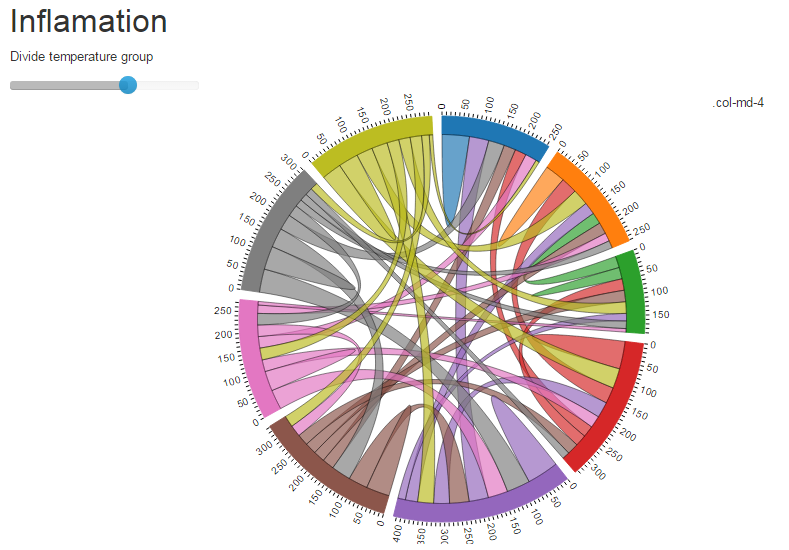
\includegraphics[width=\textwidth]{images/chordDiagram.PNG}
    \caption{the visualization with only the slider ander the chord diagram visible}
    \label{fig:overView}
\end{figure}
\newpage
\section{Description of the Dataset}
We have been given a dataset with information about certain patients and certain diseases that ales them. The data is provided in a .csv file with 120 rows and 8 columns every column is separated by a tab. Every row represents a patient. There is also a .txt file with a more detailed explanation of how the data in the .csv can be read.
\subsection{High-level description}
Our data set is called "inflammation.csv" and it describes patients and the diseases that ales them. There are 8 columns that represent the diseases and there are 120 rows that represent the patients. The data from the 2nd to the 8th column are "yes" to indicate that he has the disease of that column or "no" to indicate that he doesn't have the disease that the column represents. For example: \newline
\textbf{'35,9 no no yes yes yes yes no'} \newline
Where: \newline
'35,9' Temperature of patient \newline
'no' Occurrence of nausea \newline
'no' Lumbar pain \newline
'yes' Urine pushing (continuous need for urination) \newline
'yes' Micturition pains \newline
'yes' Burning of urethra, itch, swelling of urethra outlet \newline
'yes' decision: Inflammation of urinary bladder \newline
'no' decision: Nephritis of renal pelvis origin  \newline

\subsection{Description of the format}
The data has been gathered from a paper about diagnosis of urinary system diseases \footnote{J.Czerniak, H.Zarzycki, Application of rough sets in the presumptive diagnosis of urinary system diseases, Artifical Inteligence and Security in Computing Systems, ACS'2002 9th International Conference Proceedings, Kluwer Academic Publishers,2003, pp. 41-51} \newline
take from the dataset: \newline
The main idea of this data set is to prepare the algorithm of the expert system, which will perform the presumptive diagnosis of two diseases of urinary system. It will be the example of diagnosing of the acute inflammations of urinary bladder and acute nephritises. For better understanding of the problem let us consider definitions of both diseases given by medics. Acute inflammation of urinary bladder is characterised by sudden occurrence of pains in the abdomen region and the urination in form of constant urine pushing, micturition pains and sometimes lack of urine keeping. Temperature of the body is rising, however most often not above 38C. The excreted urine is turbid and sometimes bloody. At proper treatment, symptoms decay usually within
several days. However, there is inclination to returns. At persons with acute inflammation of urinary bladder, we should expect that the illness will turn into protracted form. \newline
Acute nephritis of renal pelvis origin occurs considerably more often at women than at men. It begins with sudden fever, which reaches, and sometimes exceeds 40C. The fever is accompanied by shivers and one- or both-side lumbar pains, which are sometimes very strong. Symptoms of acute inflammation of urinary bladder appear very often. Quite not infrequently there are nausea and vomiting and spread pains of whole abdomen. \newline
The data was created by a medical expert as a data set to test the expert system, which will perform the presumptive diagnosis of two diseases of urinary system. The basis for rules detection was Rough Sets Theory. Each instance represents an potential patient. \newline
Attribute Information: \newline
a1 Temperature of patient \{ 35C-42C \} \newline
a2 Occurrence of nausea \{ yes, no \} \newline
a3 Lumbar pain \{ yes, no \} \newline
a4 Urine pushing (continuous need for urination) \{ yes, no \} \newline
a5 Micturition pains \{ yes, no \} \newline
a6 Burning of urethra, itch, swelling of urethra outlet \{ yes, no \} \newline
d1 decision: Inflammation of urinary bladder \{ yes, no \} \newline
d2 decision: Nephritis of renal pelvis origin \{ yes, no \} \newline
\subsection{Data Representation}
With the visualization you can try to find correlations between combinations of diseases and temperature, taken from the dataset inflammation.csv. this is supposed to be used by a person who has knowledge off the data being visualized so that person knows what to select and what to analyze. We hope we have provide ample visualization techniques and provided the right amount of filter techniques for them for people with knowledge to find correlations, since both of us don't have knowledge on this subject and what would be more important to visualize.
\newpage
\section{Design}
In this section we explain the general design of the visualization.
\subsection{General design}
What the goal is with the visualization is finding a correlation between the data, for instance between the temperature and the diseases that the patients tend to have. For this we used a bar chart, a chord diagram and parallel coordinates. We also implemented a slider that allows the user to determine a temperature range for which the data will be visualized.
\subsection{User Interface}
The ways we've decided to represent the data will be all shown on the page and there will be a slider that affects all visualizations, so the data is connected. A more detailed description of the visualization methods can be found in the implementation chapter. \newline
All the data is shown on top of each other so each of them can be accessed. At the top is the chord diagram, you can select a part of the chord diagram and the lines of that part will be lit up. Below there you see the parallel coordinates, you can select a line or a selection of lines to see how they maneuver through the graph, you can also reposition the bars of the parallel coordinates to your liking. Below there you can see the bar graph, this just represents the percentage of people that have a disease from the dataset.
\newpage
\section{Implementation}
We decided to do the implementation in HTML, CSS and Javascript, the reasoning for this is because this way users will be able to visi the visualization easily using their web-browser, without needing to install additional software. \newline
For the visualization of data, we used the d3.js library. This library allows users o handle data in Javascript easily. for the visualization we also used the scripts dimple.js, which uses the d3.js library and allows you take full advantage of the power of d3 to visualize data. In the end with d3 we made a parallel coordinates, chord diagram and a bar chart that use the dataset provided.
\subsection{Technical Notes}
We have tested the application in Firefox and Chrome. Other modern browsers like Safari, Opera and Internet Explorer should also support our application, but we have not tested that.
\subsection{Main Interface}
The main view will be all visualizations below each other with the chord diagram on top, below the parallel coordinates and under that the bar chart, there will be a slider visible on the top of the page on which you can select a temperature range that will filter the data used in the visualizations. These will than update with the filtered data.
\newpage
\subsection{Parallel Coordinates}
We used the dataset that was provided to visualize it in a parallel coordinates visualization. Parallel coordinates are one of the most famous visualization techniques, and among the most common subjects of academic papers in visualization. While initially confusing, they are a very powerful tool for understanding multi-dimensional numerical datasets. \newline
For instance now can be seen that a high temperature and nausea have a direct connection. The full result of this can be seen in figure \ref{fig:Parallel}.
\begin{figure}[h]
\begin{center}
    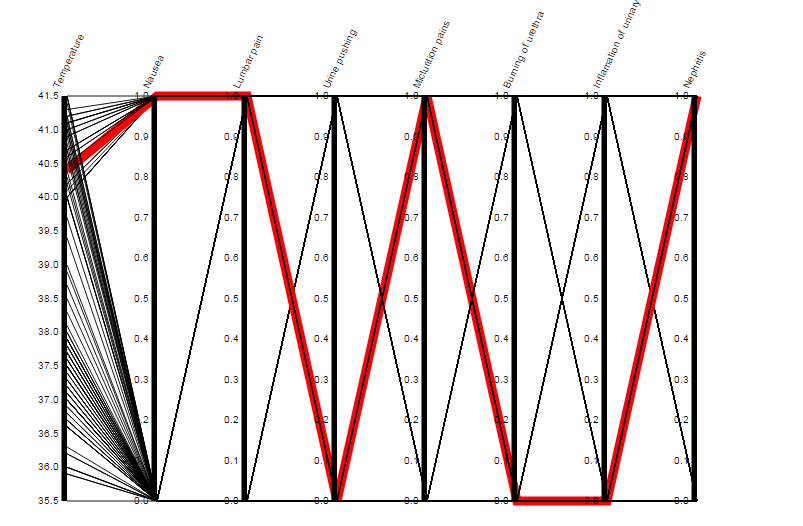
\includegraphics[width=0.8\textwidth]{images/ParallelCoordinates.PNG}
    \caption{the parallel Coordinates visualization}
    \label{fig:Parallel}
\end{center}
\end{figure}
\newpage
\subsection{Bar Chart}
The Bar Chart uses vertical bars to show comparisons among the disease categories. on the x axis the different diseases from the dataset are represented and on the y axis the percentage of people that have it is displayed. The percentage is based on the amount of people that are in the dataset and on which percentage has the disease, for each disease there is a bar. This is a basic technique, but it is very useful to see which diseases are more prevalent among the people. The full result of this can be seen in figure \ref{fig:Bar}.
\begin{figure}[h]
\begin{center}
    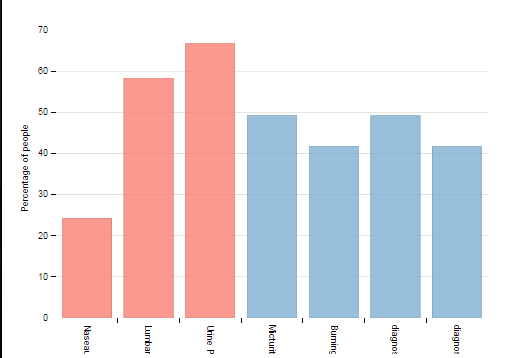
\includegraphics[width=0.8\textwidth]{images/barChart.PNG}
    \caption{the Bar Chart visualization}
    \label{fig:Bar}
\end{center}
\end{figure}
\newpage
\subsection{Chord Diagram}
A chord diagram is a graphical method of displaying the inter-relationships between data in a matrix. The data is arranged radially around a circle with the relationships between the points drawn as arcs connecting the data together. The full result of this visualization can be seen in figure \ref{fig:Chord}\newline
\begin{figure}[h]
\begin{center}
    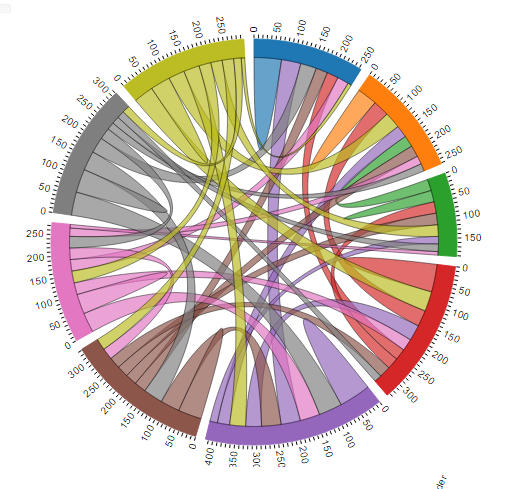
\includegraphics[width=0.8\textwidth]{images/chordDiagramSolo.PNG}
    \caption{the Chord Diagram visualization}
    \label{fig:Chord}
\end{center}
\end{figure}
\newpage
\subsection{Hovering and Selecting}
To get more detail from a particular visualization, the user can hover over it with the mouse, this has an effect on every visualization. \newline
With the chord diagram, just that part of the circle and the relations are highlighted so you can more easily see the relations. \newline
With the parallel coordinates when you hover over a line, it will be highlighted red all along the graph, so you can see how it traverses the graph. \newline
With the bar chart more information of the bar is given if it is hovered over, it will display the full name on the x axis of the disease and also the percentage in a label located at the mouse.
\end{document} 